\documentclass[conference,12pt,onecolumn]{IEEEtran}
\usepackage[a4paper, left=2.5cm, right=2.5cm, bottom=2cm, top=2.5cm]{geometry}
\usepackage{graphicx}
\usepackage[utf8]{inputenc}

\usepackage{makecell}
% Some very useful LaTeX packages include:
% (uncomment the ones you want to load)


% *** MISC UTILITY PACKAGES ***
%
%\usepackage{ifpdf}
% Heiko Oberdiek's ifpdf.sty is very useful if you need conditional
% compilation based on whether the output is pdf or dvi.
% usage:
% \ifpdf
%   % pdf code
% \else
%   % dvi code
% \fi
% The latest version of ifpdf.sty can be obtained from:
% http://www.ctan.org/pkg/ifpdf
% Also, note that IEEEtran.cls V1.7 and later provides a builtin
% \ifCLASSINFOpdf conditional that works the same way.
% When switching from latex to pdflatex and vice-versa, the compiler may
% have to be run twice to clear warning/error messages.






% *** CITATION PACKAGES ***
%
%\usepackage{cite}
% cite.sty was written by Donald Arseneau
% V1.6 and later of IEEEtran pre-defines the format of the cite.sty package
% \cite{} output to follow that of the IEEE. Loading the cite package will
% result in citation numbers being automatically sorted and properly
% "compressed/ranged". e.g., [1], [9], [2], [7], [5], [6] without using
% cite.sty will become [1], [2], [5]--[7], [9] using cite.sty. cite.sty's
% \cite will automatically add leading space, if needed. Use cite.sty's
% noadjust option (cite.sty V3.8 and later) if you want to turn this off
% such as if a citation ever needs to be enclosed in parenthesis.
% cite.sty is already installed on most LaTeX systems. Be sure and use
% version 5.0 (2009-03-20) and later if using hyperref.sty.
% The latest version can be obtained at:
% http://www.ctan.org/pkg/cite
% The documentation is contained in the cite.sty file itself.






% *** GRAPHICS RELATED PACKAGES ***
%
\ifCLASSINFOpdf
  % \usepackage[pdftex]{graphicx}
  % declare the path(s) where your graphic files are
  % \graphicspath{{../pdf/}{../jpeg/}}
  % and their extensions so you won't have to specify these with
  % every instance of \includegraphics
  % \DeclareGraphicsExtensions{.pdf,.jpeg,.png}
\else
  % or other class option (dvipsone, dvipdf, if not using dvips). graphicx
  % will default to the driver specified in the system graphics.cfg if no
  % driver is specified.
  % \usepackage[dvips]{graphicx}
  % declare the path(s) where your graphic files are
  % \graphicspath{{../eps/}}
  % and their extensions so you won't have to specify these with
  % every instance of \includegraphics
  % \DeclareGraphicsExtensions{.eps}
\fi
% graphicx was written by David Carlisle and Sebastian Rahtz. It is
% required if you want graphics, photos, etc. graphicx.sty is already
% installed on most LaTeX systems. The latest version and documentation
% can be obtained at:
% http://www.ctan.org/pkg/graphicx
% Another good source of documentation is "Using Imported Graphics in
% LaTeX2e" by Keith Reckdahl which can be found at:
% http://www.ctan.org/pkg/epslatex
%
% latex, and pdflatex in dvi mode, support graphics in encapsulated
% postscript (.eps) format. pdflatex in pdf mode supports graphics
% in .pdf, .jpeg, .png and .mps (metapost) formats. Users should ensure
% that all non-photo figures use a vector format (.eps, .pdf, .mps) and
% not a bitmapped formats (.jpeg, .png). The IEEE frowns on bitmapped formats
% which can result in "jaggedy"/blurry rendering of lines and letters as
% well as large increases in file sizes.
%
% You can find documentation about the pdfTeX application at:
% http://www.tug.org/applications/pdftex





% *** MATH PACKAGES ***
%
%\usepackage{amsmath}
% A popular package from the American Mathematical Society that provides
% many useful and powerful commands for dealing with mathematics.
%
% Note that the amsmath package sets \interdisplaylinepenalty to 10000
% thus preventing page breaks from occurring within multiline equations. Use:
%\interdisplaylinepenalty=2500
% after loading amsmath to restore such page breaks as IEEEtran.cls normally
% does. amsmath.sty is already installed on most LaTeX systems. The latest
% version and documentation can be obtained at:
% http://www.ctan.org/pkg/amsmath





% *** SPECIALIZED LIST PACKAGES ***
%
%\usepackage{algorithmic}
% algorithmic.sty was written by Peter Williams and Rogerio Brito.
% This package provides an algorithmic environment fo describing algorithms.
% You can use the algorithmic environment in-text or within a figure
% environment to provide for a floating algorithm. Do NOT use the algorithm
% floating environment provided by algorithm.sty (by the same authors) or
% algorithm2e.sty (by Christophe Fiorio) as the IEEE does not use dedicated
% algorithm float types and packages that provide these will not provide
% correct IEEE style captions. The latest version and documentation of
% algorithmic.sty can be obtained at:
% http://www.ctan.org/pkg/algorithms
% Also of interest may be the (relatively newer and more customizable)
% algorithmicx.sty package by Szasz Janos:
% http://www.ctan.org/pkg/algorithmicx




% *** ALIGNMENT PACKAGES ***
%
%\usepackage{array}
% Frank Mittelbach's and David Carlisle's array.sty patches and improves
% the standard LaTeX2e array and tabular environments to provide better
% appearance and additional user controls. As the default LaTeX2e table
% generation code is lacking to the point of almost being broken with
% respect to the quality of the end results, all users are strongly
% advised to use an enhanced (at the very least that provided by array.sty)
% set of table tools. array.sty is already installed on most systems. The
% latest version and documentation can be obtained at:
% http://www.ctan.org/pkg/array


% IEEEtran contains the IEEEeqnarray family of commands that can be used to
% generate multiline equations as well as matrices, tables, etc., of high
% quality.




% *** SUBFIGURE PACKAGES ***
%\ifCLASSOPTIONcompsoc
%  \usepackage[caption=false,font=normalsize,labelfont=sf,textfont=sf]{subfig}
%\else
%  \usepackage[caption=false,font=footnotesize]{subfig}
%\fi
% subfig.sty, written by Steven Douglas Cochran, is the modern replacement
% for subfigure.sty, the latter of which is no longer maintained and is
% incompatible with some LaTeX packages including fixltx2e. However,
% subfig.sty requires and automatically loads Axel Sommerfeldt's caption.sty
% which will override IEEEtran.cls' handling of captions and this will result
% in non-IEEE style figure/table captions. To prevent this problem, be sure
% and invoke subfig.sty's "caption=false" package option (available since
% subfig.sty version 1.3, 2005/06/28) as this is will preserve IEEEtran.cls
% handling of captions.
% Note that the Computer Society format requires a larger sans serif font
% than the serif footnote size font used in traditional IEEE formatting
% and thus the need to invoke different subfig.sty package options depending
% on whether compsoc mode has been enabled.
%
% The latest version and documentation of subfig.sty can be obtained at:
% http://www.ctan.org/pkg/subfig







% *** PDF, URL AND HYPERLINK PACKAGES ***
%
%\usepackage{url}
% url.sty was written by Donald Arseneau. It provides better support for
% handling and breaking URLs. url.sty is already installed on most LaTeX
% systems. The latest version and documentation can be obtained at:
% http://www.ctan.org/pkg/url
% Basically, \url{my_url_here}.




% *** Do not adjust lengths that control margins, column widths, etc. ***
% *** Do not use packages that alter fonts (such as pslatex).         ***
% There should be no need to do such things with IEEEtran.cls V1.6 and later.
% (Unless specifically asked to do so by the journal or conference you plan
% to submit to, of course. )


% correct bad hyphenation here
\hyphenation{op-tical net-works semi-conduc-tor}


\begin{document}
%
% paper title
% Titles are generally capitalized except for words such as a, an, and, as,
% at, but, by, for, in, nor, of, on, or, the, to and up, which are usually
% not capitalized unless they are the first or last word of the title.
% Linebreaks \\ can be used within to get better formatting as desired.
% Do not put math or special symbols in the title.
\title{Vehicle-to-Everything Communications (V2X) in 5G}


% author names and affiliations
% use a multiple column layout for up to three different
% affiliations
\author{\IEEEauthorblockN{Hugo Rummlinger, Frederik Schulz, Theo Mamone, Anthony Dell'Eva}
\IEEEauthorblockA{Universitat Politècnica de Catalunya\\
Master degree in Telecommunications Engineering\\
5G Mobile Communication Systems}}


% make the title area
\maketitle

\begin{abstract}
In the abstract, you write 2-3 paragraphs which summarize the key parts of your report.
\end{abstract}


\IEEEpeerreviewmaketitle

\section{Papers Used \& How To Cite Them}
\begin{itemize}
\item V2X access technologies: Regulation, research, and remaining challenges [Cite: machardy2018] \cite{machardy2018}
\item Dedicated short-range communications (DSRC) standards in the United States [Cite: kenney2011] \cite{kenney2011}
\item Standards for vehicular communication---from IEEE 802.11p to 5G [Cite: festag2015]\cite{festag2015}
\item Ready to roll: Why 802.11 p beats LTE and 5G for V2x [Cite: filippi2016] \cite{filippi2016}
\item Heterogeneous Vehicular Networking: A Survey on Architecture, Challenges, and Solutions [Cite: zheng2015] \cite{zheng2015}
\item LTE-advanced in 3GPP Rel -13/14: an evolution toward 5G [Cite: lee2016] \cite{lee2016}
\item LTE for vehicular networking: a survey [Cite: araniti2013] \cite{araniti2013}
\item Use cases, requirements, and design considerations for 5G V2X [Cite: boban2017] \cite{boban2017}
\item Design aspects for 5G V2X physical layer [Cite: boban2016] \cite{boban2016}
\item Non-Orthogonal Multiple Access for High-Reliable and Low-Latency V2X Communications in 5G Systems [Cite: di2017] \cite{di2017}
\item  LTE evolution for vehicle-to-everything services [Cite: seo2016] \cite{seo2016}
 \item Device-to-device communications; functional prospects for LTE-advanced networks [Cite: doppler2009] \cite{doppler2009}
  \end{itemize}

\section{Introduction}
- Cooperative intelligent transportation systems (C-ITS) gained a lot of interest from different groups. V2X, short for Vehicle to Everything communication, is a specific case of ITS, dealing with wireless communication and coordination between vehicles and their environment.
- V2X can be taken in this paper to refer specifically to communication between overland road vehicles and other con- cerned entities, be they pedestrians, infrastructure, or other vehicles. \cite{machardy2018}
- Communication in V2X cases happens in a frequently changing vehicular ad-hoc networks (VANET)s, where nodes of the network leave and join the network at a specific location as frequently as the traffic floads. This VANET is supported by a static network. Nodes of this network a typically referred to as road side units (RSU), helping to coordinate non-static nodes communication traffic, distributing data and providing additional services \cite{machardy2018}.
- V2X technology tries to increase safety, efficiency and reduce economic costs of the current and future transportation system. \cite{machardy2018}

\begin{figure} [ht]
   \centering
   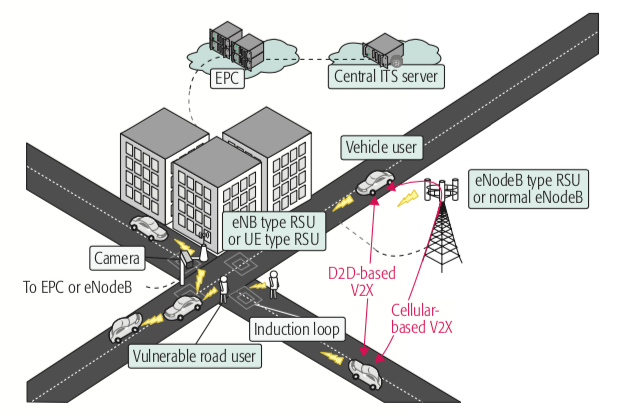
\includegraphics[width=0.7\linewidth]{_Graphics/v2x_deployment_example.png}
  \caption{V2X Deployment Scenario. \cite{seo2016}}
  \label{fig:v2x_deployment_example}
\end{figure}

\section{Use-Cases} use \cite{boban2017} for 5G requirements and \cite{5gamericas2018} pag.24
\subsection{Vehicle-to-Vehicle}
\subsection{Vehicle-to-Infrastructure/Network}
\subsection{Vehicle-to-Person}


\begin{table}[h!]
  \begin{center}
  \caption{V2X Services Grouped into Four Major Categories \cite{machardy2018} - Applications and Requirements}
    \label{tab:V2X_services}
    \begin{tabular}{ccc}
      \textbf{\makecell{Service}} & \textbf{\makecell{Applications}} & \textbf{Requirements} \\
      \hline
      \textbf{\makecell{Infotainment}}& \makecell[c]{Geo-related advertisement\\ Messaging \\ Media transfer (i.e. Netflix)\\} & \makecell[c]{Low requirement for latency\\ (500-1000 ms)\\ Transm. frequency around 1 Hz\\ Throughput around 80 Mbps}\\
      \\
      \textbf{\makecell{Traffic Efficiency}}& \makecell[c]{Optimizing traffic flow \\ Intersection timing \\ Real time route planning} & \makecell[c]{Constant information exchange\\ Usually not safety critical\\ Medium latency \\ Medium throughput} \\
      \\
      \textbf{\makecell{Traffic Safety}}& \makecell[c]{Reduce collsions \\ Reduce impact of collisions \\(Costs and casualties)} & \makecell[c]{Need for critical decisions\\Ultra reliable robust network\\ High latency and Throughput} \\
      \\
       \textbf{\makecell{Cooperative Driving}}& \makecell[c]{Cruise control\\ Cooperative platooning} & \makecell[c]{High frequency of exchange\\ Low latency (2-10 ms)\\ Throughput: Depends on use-case\\}\\
    \end{tabular}
  \end{center}
\end{table}

\section{V2X in LTE Networks}
The possibility for V2X communication is firstly regarded an option in LTE for cellular networks. With an increasing densification of the cellular network and the growing capacity of LTE networks, V2X over cellular networks seemed to be a perfect choice at first sight. In the following we describe the current situation regarding V2X and LTE, highlighting the nature of V2X communication and the consequent problems for the current cellular network infrastructure.

\begin{figure} [ht]
   \centering
   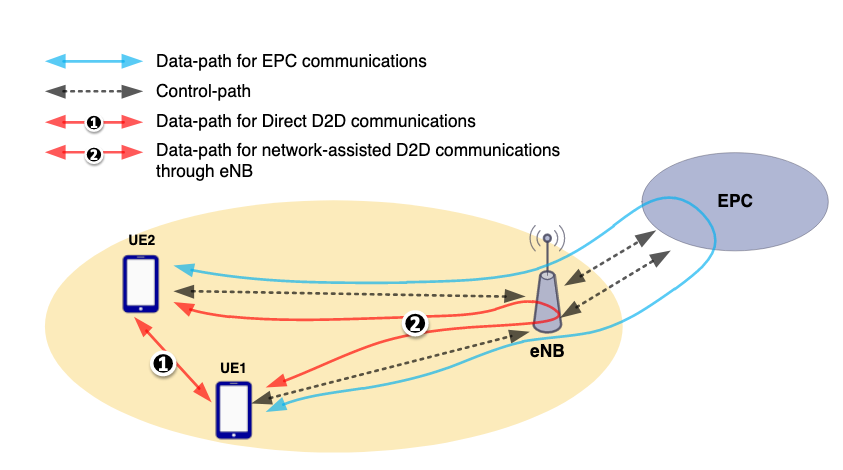
\includegraphics[width=0.7\linewidth]{_Graphics/lte_d2d_usecases.png}
  \caption{Possible D2D Connection Scenarios in LTE. \cite{gunes2014}}
  \label{fig:lte_d2d_usecases}
\end{figure}

LTE based systems offer to possibilities for V2X communication. Devices can either use direct D2D communication over the PC5 interface or use the E-UTRAN interface to connect to an eNB, shown as the red connections and the blue connection in figure \ref{fig:lte_d2d_usecases}. Furthermore these two options offer two ways to establish a connection. Every type of connection has its own properties. D2D communication typically allows for an direct connection between UE's in each other proximity. D2D connections offers two modes. One mode allows for an direct connection without the need of an eNB and is typically used when there is no network infrastructure close by (See figure \ref{fig:lte_d2d_usecases} red connection annotated with a 1). Hereby the UE's autonomously select resources to use for communication from an pool of frequencies know upfront and schedule their transmissions in an distributed manner. This kind of communication is similar to Wi-Fi and not naturally used in cellular networks therefore introducing additional protocols and sensing otherwise not used. The other mode offers an logical D2D communication by establishing an connection to another device via an eNB (See figure \ref{fig:lte_d2d_usecases} red connection annotated with a 2). As this procedure allows to use the natural cellular scheduling and allocation techniques but comes with the need of infrastructure. Additionally in contrast to direct D2D connections, an active RRC connection is needed in this case. Typically direct communication would only be used in case of missing eNB connectivity, but as most vehicular transmissions nature is of packages of small size but in heavy frequencies, this approach could ease the load for the infrastructure.
The E-UTRAN interface also allows for two possible connection types. Packets can be transmitted via the normal physical uplink shared channel (PUSCH) and physical downlink shared channel (PDSCH) or use the evolved multimedia broadcast multicast service (eMBMS). If the communication takes place via D2D or the E-UTRAN depends on the situation and can be changed for downlink and uplink independently, making the system flexible.

\begin{figure} [ht]
   \centering
   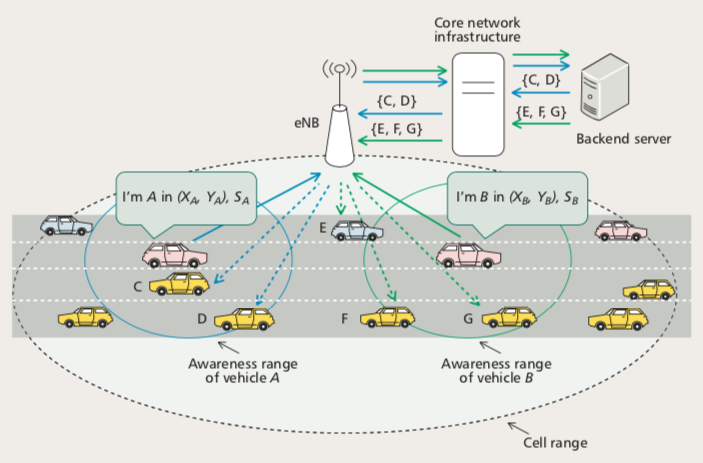
\includegraphics[width=0.6\linewidth]{_Graphics/lte_backendserver.png}
  \caption{Multicast CAM Delivery in LTE with Backend Server Coordinating Awareness Range. \cite{araniti2013}}
  \label{fig:lte_backendserver}
\end{figure}

V2X communication foresees the periodic transmission of different data from an UE to the network and other UE. This includes speed, next action and different sensor data, like street condition, sight and so forth. Naturally these kind of information are not useful for every UE in the network. Therefore the ETSI defines the need for a special-purpose backend server \cite{araniti2013}. This server will take care of keeping a list where each UE is located in the network and other services like intelligent data analysis. As the server is aware where the devices are located geographically it can take incoming traffic from messages and redistribute them to vehicles who are in close proximity or for whom the information is valuable. An advanced case could be, if a car is scheduled to drive through an area of increasing traffic or where an accident happened, the server could notify the cars navigation system to use a different route. The backend server is a key element to fulfil future applications goals \cite{araniti2013}. There are two possible options how an backend server can be deployed. The first one is to deploy the server directly in the EPC network itself, this would allow the server to take the geographical information directly from the MME module inside the network. The second option is to deploy the server in the internet. The first option would reduce the amount of connections going through the network, as an server deployed in the internet would introduce the need of one active connection per UE to the server. In contrast to the MME module which even samples geographical data when the UE is in idle mode. To make use of this intelligent system most messages need to go through the network \cite{araniti2013} to allow for the backend server to analyse the data.

\begin{table}[h!]
  \begin{center}
  \caption{V2V Message Types - Requirements and Applications. (Defined by ETSI) \cite{araniti2013}}
    \label{tab:message_types}
    \begin{tabular}{lll}
      \textbf{\makecell{Message}} & \textbf{\makecell{Requirements}} & \textbf{\makecell{Applications}} \\
      \hline
      \textbf{\makecell{Cooperative Awareness\\  Messages - CAM's}}& \makecell[c]{Periodic time-triggered \\ Frequency: 1 - 10 Hz \\ Max. latency: 100 ms \\ Length: 800 bytes}& \makecell[c]{Emergency vehicle warning \\ Slow vehicle indication \\ Intersection collision warning \\ Motorcycle approaching indication \\ Collision risk warning \\ Speed limits notification \\ Traffic light optimal speed advisory}\\ \\
      \textbf{\makecell{Decentralized Environ-\\mental Notification\\ Messages - DENM's}}& \makecell[c]{Event driven warnings\\ Max. latency: 100 ms\\ Length: Shorter than CAM's}& \makecell[c]{Emergency electronic light warning\\ Wrong way driving warning\\ Stationary vehicle accident \\ Traffic condition warning\\ Signal violation warning\\ Road work warning\\ Collision risk warning\\}\\
    \end{tabular}
  \end{center}
\end{table}

The two message types defined by the ETSI which are concerned with transmitting status updates and emergency information are called cooperative awareness message (CAM) and decentralized environmental notification message (DENM). CAM's are of periodic nature and introduce the most load to the network, DENM's on the other side occur in warning and emergency situations (Cf. table \ref{tab:message_types}). The traffic characteristics of CAM's and the need for latency for both CAM's and DENM's are challenging for LTE based networks \cite{seo2016}.
LTE V2X foresees the usage of eMBMS to ease the load of the network and lower the amount of connections. Hereby vehicles would still use single connections in the uplink to distribute their CAM and DENM to network. As these messages will in most cases be filled with redundant information an intelligent server could accumulate the information and only redistribute a single message or an drastically lower amount of messages back to the vehicles, for whom the information are relevant. The nature of eMBMS if perfectly suited for this purpose at it allows for geographically restricted single to multipoint communications and even takes advantage of redundant transmissions of multiple eNB's \cite{araniti2013} resulting also in an lower latency.
On the downside eMBMS needs an active session to be used, which could permit the usage of the same as latency is increased and might be to high as session setup takes time and one can not hold an active session all the time \cite{lee2016}. An example of the usage of eMBMS connections, an backend server which redistribute CAM's can be seen in figure \ref{fig:lte_backendserver}. As one can see, the received messages are sent through the network to the server, and after beeing analysed are send to the vehicles for whom the information is useful via eMBMS connections. As already mentioned above, the transmission characteristics of V2X communication, not taking into account infotainment services, is different to the common LTE services providing for example voice or message communication. Cars need to propagate their updated position, speed and sensor data, to name a few, periodically in the network (Cf. figure \ref{tab:message_types} CAM messages).These periodic messages can introduce a heavy load to the network especially in cities and at rush hours and does challenge the capacities of the LTE network. As a result limiting or preventing the usage of other services \cite{araniti2013}.

Summarizing it can be seen that while LTE already allows for V2X communication there are many challenges to overcome. LTE is already applicable for V2I/N communication \cite{seo2016} and can already serve infotainment applications as proven by mobile phones, with limitations on availability. Improvement is needed in D2D communication, as LTE D2D communication was primary developed for voice calls with tens of users in mind not hundreds \cite{seo2016}. Furthermore the current system is not properly capable of handling Doppler effects, frequency errors and inter-carrier interference at high velocity of vehicles in every scenario, i.e. crossing vehicles on highways \cite{seo2016}. It can be stated that a future network need to be able to cope with high vehicle speed and high UE density which will be a main technical challenge \cite{seo2016} and to handle high loads of periodic messages without loosing its capability to serve other services \cite{lee2016} which at the moment is not possible \cite{lee2016}. Also for a save V2X communication the cellular network need to be able to handle handovers in a way, that they do not introduce significant latency, which otherwise leads to time with no communication abilities beeing dangerous as a result \cite{seo2016}.

\section{Evolution from LTE to 5G}
- maybe use \cite{lee2016}
- maybe use  \cite{boban2017}
- maybe use \cite{boban2016}
- maybe use \cite{di2017}

The following section describes the main network evolutions introduced by 5G in order to support new services and requirements. Starting from a brief overview of the novel architectural principles, the attention is then focused on the applications of the new paradigms to the V2X scenario.

The need for an LTE EPS enhancement toward a flexible mobile architecture has been triggered by the birth of new services such as Internet of Things (Iot), eHealth and, precisely, Vehicular-to-everything (V2X). Maintaining backward compatibility, the evolved architecture must support not only legacy radio technologies, but also new radio access methodologies such as millimetre-wave (mmWave) transmissions. Furthermore, it has to be able to integrate different processing models such as cloud RAN (C-RAN) and mobile edge computing (MEC), while allowing deployments  based on microcells and macrocells and the support to very diverse use cases and requirements in terms of throughput and latency, as explained in the above sections.

The fundamental objectives, which are the multi-service and context-aware adaptation and the multi-tenancy of the mobile network, are achieved thanks to the following functionalities \cite{rost2016mobile}:
\begin{itemize}
\item \textbf{Network of functions}: the architecture is service-based, i.e. the specification focuses on the services rather than the nodes. This is in  line with the use of NFV (Network Function Virtualization) for implementing core network functions.
\item \textbf{Network slicing}: the infrastructure is flexible and can be customized thanks to different virtual subnetworks optimized for the specific use case.
\item \textbf{Software-defined mobile network}: programmable control of a flexible network of functions as well as a set of network slices. This allows to adapt the network behaviour to the current requirements. It is in line with the split of the control and user planes, which enables independent and scalability evolution.
\end{itemize}

\subsection*{New radio technologies}
The novel radio technologies that are envisioned as components of a 5G network providing V2X services and which should be integrated with the technologies already exploited in LTE such as Cellular V2X (LTE-V) and DSCR (IEEE 802.11p protocol suite), are the following \cite{boban2017}:
\begin{itemize}
\item \textbf{Millimeter-wave communication}. It is very attractive from the data throughput point of view but it has crucial challenges on the physical layer perspective, due to its high propagation path loss and its sensitivity to shadowing. Furthermore, in the 50-60 GHz band, the Doppler effect is a major drawback since it is linear in the carrier frequency: new solutions have to be set up, such as special frame design and numerology. 

These effects make the mmWave communication suitable for mostly short range (not more than few hundred meters) and point to point line of sight (LOS) transmissions \cite{rangan2014millimeter}. In particular, it can bring advantages for both V2I communications, establishing short-timed high data rates connections in order to exchange information which are insensitive to delay, such as traffic data for large scale traffic monitoring in the uplink and infotainment data and maps updates in the downlink, and V2V communications, supporting the exchange of messages between vehicles in a platoon \cite{va2016millimeter}. In fact, radio signals can be used for position estimation: the achievable accuracy for 5G networks is considerably higher than the one achievable for legacy LTE networks, thanks to the higher signal bandwidth and the deployments based on micro cells, which make the network nature denser and enable LOS with high probability.


\item \textbf{Vehicular Visible Light Communication (VVLC)}. Even if not direcly correlated to the evolution of the 5G networks and their relative technologies, VVLC could be introduced in the new V2X solutions.

 VVLC configuration is composed by light emitting diodes (LEDs) in vehicles headlights and taillights, which are used to transmit information, and by photo diodes or cameras, which work as receivers. The cost of adding VVLC capability to cars is limited to only inexpensive circuitry that permits the communication. This makes it suitable for low cost installations as, for example, scooters or cheap cars that cannot cover expensive systems in the price. Furthermore, VVLC has centimeter-precision relative positioning capability, thanks to the dual configuration (headlight/taillight) and the known dimensions of the vehicles \cite{roberts2010}, which is exploited as a useful complement to satellite-based positioning systems, that have only meter-precision capability. This characteristic makes the technology suitable for manoeuvres which require high precision positioning, such as parking.

The performances include a range of 50m and a bitrate up to 2 Mb/s at 50m and more than 500 Mb/s at 5m \cite{yu2013}. Finally, the separated configuration of transmitter (LEDs) and receiver (photo diode/camera), enables full duplex communication.
\end{itemize}

\cite{5gamericas2018}








\section{Other Access Technologies}
The following section deals with access technologies for V2X communication besides or in cooperation with cellular networks. We will only refer to the access technologies itself, if at all mentioning the eventually necessary infrastructure only briefly.
\subsection{Dedicated Short Range Communication}
Most scientific papers refer to dedicated short range communication (DSRC) as systems using IEEE 802.11p and  IEEE 1609 (WAVE) standards together for communication\cite{machardy2018}. Hereby the 802.11p standard allows for a setup of vehicular ad-hoc networks (VANET's) taking care of the physical (PHY) layer and the medium access (MAC) layer while the WAVE standard defines networking and some application related parts like security and authentication.
As an amendment to the Wi-Fi specification 802.11 defined by the IEEE organisation, 802.11p allows for inter device communication and is especially developed with V2X communication in mind. It facilitates the communication without the usual need for an basic service set (BSS, e.g. access point or something similar), allowing for D2D communication without a central coordinator \cite{machardy2018}. The standard itself does not define a specific operational frequencies, rather it defines the procedure of communication, leaving the choice of the used frequency to the authorities. As requirements for in V2X communication differ highly from typical Wi-Fi communication, 802.11p introduces a new medium access method called tiered contention multiple access (TMAC). This MAC technique allows for a prioritization of messages which is not possible with the typically used CSMA/CA technique \cite{machardy2018}. Especially for safety critical messages, relate to traffic safety like pre-crash sensing a prioritization of data flows is essential.
As with most wireless communications synchronization is needed for communication in DSRC \cite{kenney2011}. With the lack of an central coordination entity routing of multi-hop is a hard task in VANET's when mobility of nodes is high. Due to the fast changing topology of the network, routes can be already obsoleted when found i\cite{machardy2018}. To which degree this affects communication depends heavily on the used routing protocol.
Another aspect in V2X communication is safety, as it is critical to have reliable communication partners. Users acting maliciously can spam the network or trying to insert wrong data into the network. DSRC uses a private key infrastructure for this aspect. Hereby a central authority distributes autonomous and temporal certificates to vehicles. Those are then used to sign messages. As malicious users can not be detected upfront there exist an entity, misbehaviour authority, which is entrusted with detecting malicious vehicles and adding them to a blacklist. For this system to work, vehicles need to regularly update their own list of blacklisted certificates. As this list can be relatively large, this system imposes requirements in terms of throughput and latency \cite{machardy2018}.

Summarizing it can be said, that DSRC allows for an low-end-to-end latency, a flexible organisation of nodes and relatively low cost for deployment in the V2X use-case. But it also entails a number of issues, including throughput problems in congestion situations, security issues and difficulties to handle non-line-of-sight communication \cite{machardy2018}. The U.S. Department of Transportation (USDOT) already specified DSRC for deployment. In the following this specification is used exemplary.

\subsubsection*{Standardization U.S. Department of Transportation}
As an exemplary standardization the following proposal of the USDOT for V2X communication is taken. As the standardization entity is the U.S. Government, the choice are not compulsory, but rather shell show how a specification for DSRC can look like.
The USDOT choose to 10 MHz channel, as a result of taken measurements. Those indicated that 10 MHz channel width is well suited to deal with delay problems and Doppler spreads \cite{kenney2011}. These have to be taken into account due to the different mobility properties of cars, compared to pedestrians.  Though safety critical messages can be faster transmitted, with respect to delay not bandwith, in broader channels (e.g. 20 MHz), those typically have more noise in vehicular environment \cite{kenney2011}.
Similar to cellular networks DSRC uses orthogonal frequency-division multiple access (OFDMA) as its multiple access transmission technique. Hereby the proposition by the USDOT proposes multiple modulation rates \ref{tab:modulation_USDOT}.

\begin{table}[h!]
  \begin{center}
    \caption{Modulation Options in DSRC 10 MHz OFDMA Channels. \cite{kenney2011}}
    \label{tab:modulation_USDOT}
    \begin{tabular}{ccccc}
      \textbf{\makecell{Modulation \\ Technique}} & \textbf{\makecell{Coded \\ Bit Rate\\ (Mbps)}} & \textbf{\makecell{Coding \\ Rate}} & \textbf{\makecell{Data Rate \\ (Mbps)}} &\textbf{ \makecell{Data Bits\\ per \\OFDMA Symbol}}\\
      \hline
      BPSK &6 & 1/2 &3 &24\\
      BPSK&6 &3/4&4.5&36\\
      QPSK&12 &1/2&6&48\\
      QPSK&12&3/4&9&72\\
      16-QAM&24&1/2&12&96\\
      16-QAM&24&3/4&18&144\\
      64-QAM&36&2/3&24&192\\
      64-QAM&36&3/4&27&216\\

    \end{tabular}
  \end{center}
\end{table}

The coding used is forward error correction (FEC), which is less effective than turbo codes and therefore lowers the bit rate but has the positive property of increasing the probability of successful decoding of messages \cite{kenney2011}. As 802.11p does not define the frequency spectrum the USDOT allocated seven 10 MHz channels in the 5.9 GHz spectrum for V2X communication purposes. One aspect the DSRC technology also changes with respect to normal Wi-Fi systems is the medium access technology. As stated above the typically used CSMA/CA technique does not allow for a prioritization of messages, making it incompatible for V2X communication, as emergency situation impose a need for fast unscheduled transmissions. Therefore TMAC is used instead. This protocol misses the beaconing, synchronization, authentication and association functions of typical MAC and leaves this functionalities open for higher layers \cite{kenney2011}, making the MAC protocol simpler. Some kind of synchronization is still needed. TMAC uses Timing Advertisment (TA) frames which allow to propagate information about the time source of the sender. To allow a prioritization of messages, TMAC allows for ``more'' important messages to access the medium with a lower backoff interval, which implicitly leads to faster access and earlier transmissions.
A further change compared to most protocol stacks is the new layer 3 protocol. While it is still possible to use the most commonly used protocols at this layer, e.g. TCP/IP (see \ref{fig:architecture_DSRC}), the USDOT mostly wants to WAVE short message protocol (WSMP) for network and transportation. The reason to change from TCP/IP is the overhead associated with it. Even a small change of header size can have an impact on performance in vehicular communication environments \cite{kenney2011} and more importantly as DSRC is vulnerable to throughput degradation in case of channel congestion, smaller packets are a way to cope with this problem\cite{machardy2018}, \cite{kenney2011}. As the description of DSRC here is only very briefly and shall serve for an easier comparison between C-V2X and DSRC, the authors refer to \cite{kenney2011} for a detailed view of a DSRC specification which includes authentication and encryption properties of messages by WAVE.

\begin{figure} [ht]
   \centering
  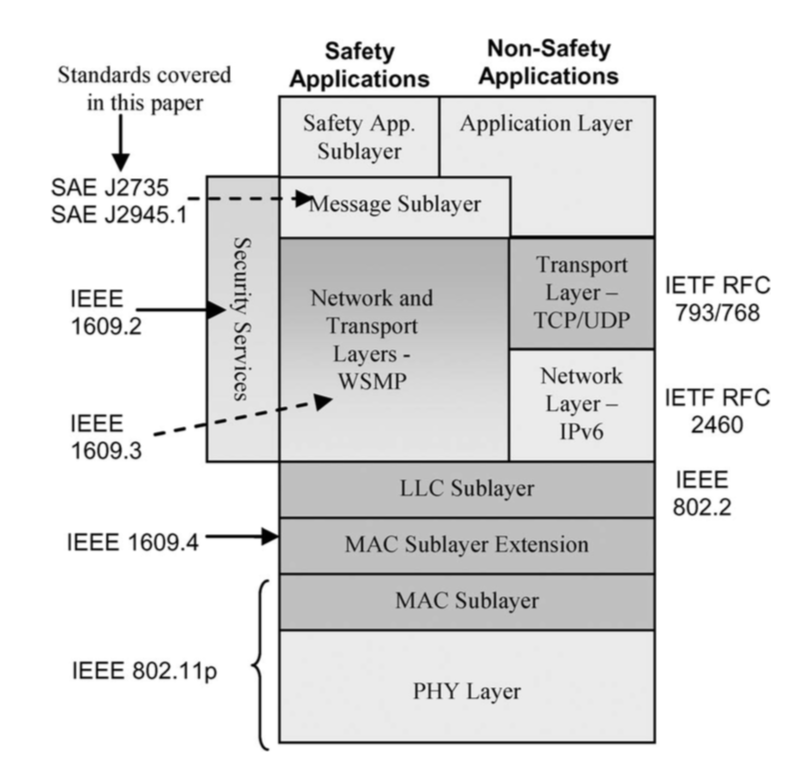
\includegraphics[width=0.5\linewidth]{_Graphics/layer_architecture_dsrc.png}
  \caption{Architecture of Layer Structure in DSRC (by USGOT). \cite{kenney2011}}
  \label{fig:architecture_DSRC}
\end{figure}

\subsection{Visible Light Communication}
\subsection{Bluetooth}

\section{Results and Discussion}
\subsection{Cellular V2X versus DSRC}
- DSRC: need for a dense deployment to cope with line of sight problems, service degradation in congestion scenarios to name a few \cite{machardy2018}
- Who will pay for theses as IEEE 802.11p networks are typically not used outside, therefore networks typically do not have access control as cellular networks \cite{machardy2018} New use case for IEEE 802.11 protocol
- DSRC mandated standard by U.S. Department of Transportation (USDOT), European Telecommunications Standards Institute (ETSI), the European Committee for Standardization (CEN) [14], and the Association of Radio Industries and Businesses (ARIB) \cite{machardy2018}
- Cellular V2X (C-V2X) Compared to DSRC, these technologies offer a number of advantages, including a much larger coverage area, pre-existing infras- tructure, deterministic security and QoS guarantees, as well more robust scalability \cite{machardy2018}
- C-V2X has on negative side: Centralized architecture, higher price for network, higher end-to-end-latency!, dependency on network connectivity \cite{machardy2018}
- Latency is a major obstacle for C-V2X deployment. Services with high need for time sensitivity, e.g. cooperative platooning or pre-crash sensing need low latency \cite{machardy2018}
- Relate here somehow to Ultra Reliable Low Latency stuff from lecture.
- How is price determined in DSRC?
- Dependency of network connectivity should be able to be done by D2D sidelink without eNB or gNB being available. Source here.
- Would D2D sidelink also solve latency issues?
- evelopment of a Channel Congestion Control
algorithm, especially for the safety channe \cite{kenney2011}
-Nonetheless, this tech- nology suffers from scalability issues, unbounded delays, and lack of deterministic quality of ser- vice (QoS) guarantees \cite{araniti2013}
- transmission range very limited, therfore need for a lot of Road Side Units (RSU) \cite{araniti2013}
- Coverage and mobility: LTE will rely on a capillary deployment of eNodeBs organized in a cellular network infrastructure offering wide area coverage \cite{araniti2013}
- higher market penetration and incentive for telecom companies to build infrastrcutre, etc. because they can get money from services offered \cite{lee2016}
- above point might also be a bad one, cause some parts of the network are safety critical and should not be non supervised by the state.
- 5G allows for different status mode of devices, where nodes are not disconnected when in idle, this reduces latency a lot and solves the issue that exist with this mode in LTE \cite{araniti2013}
- Boradcasting in 802.11p is done via one single transmission in VANET, while in LTE network (5G I do not know) this is not possible. options are a) v2v for every car in proximity (latency probably to high, because of need for estabhlishing communication first) or b) via infrastructure, but then also the infrastructure will need to distribute the messages to relevant cars in proximity. \cite{araniti2013}
- Meanwhile, effective business models should be specified to support the widespread use of LTE for cooperative ITS applications. No one would agree to pay unless highly reliable safety services and attractive traffic applications can be provided. \cite{araniti2013} Might also hold for 5G. No expensive hardware and traffic cost for signalign will be accepted if there is no use
- The central back end server can aggegrate knowledge out of multiple messages received, which is a strengt of the centralized system architecture \cite{araniti2013}

\begin{table}[h!]
  \begin{center}
  \caption{Summary of Challenges for C-V2X and 802.11p-based DSRC. \cite{machardy2018}}
    \label{tab:summary_challenges_C-V2X_DSRC}
    \begin{tabular}{lll}
      \textbf{\makecell{KPI}} & \textbf{\makecell{802.11p-based DSRC}} & \textbf{\makecell{Cellular V2X}} \\
      \hline
      \textbf{Latency}&{\tiny \makecell*[{{p{6.5cm}}}]{Not a cause for concern for 802.11p-based DSRC under normal operating conditions. An elevated packer error rate and the consequent need to retransmit messages can cause increased latency under sub-optimal conditions}}&{\tiny \makecell*[{{p{6.5cm}}}]{When operating through infrastructural nodes (e.g. eNB,EPC), processing delay is potentially problematic. Sidelink D2D and the provision of local edge resources are potential solutions to the problem of high latency}}\\
      \textbf{Capacity}&{\tiny \makecell*[{{p{6.5cm}}}]{Vehicular traffic congestion (several hundred vehicles within a 300m radius) can quickly cause high channel congestion and severely impact packer error rate. A potential path toward solving congestion issues may lie in improved congestion control schemes and controlling rate of transmissions. Optimal data-rates in the ballpark of 6 to potentially 27 Mbps are troublingly low, and may be insufficient to support many forthcoming V2X applications}}&{\tiny \makecell*[{{p{6.5cm}}}]{Depending on the size of the cell, frequent unicast transmissions via eNB from hundreds of vehicles can cause significant congestion. Using eMBMS or sidelink D2D may solve this problem. 5G aims to support data-rates measured in Gbps, which should be sufficient for all considered V2X applications}}\\
      \textbf{Coverage}&{\tiny \makecell*[{{p{6.5cm}}}]{LOS and relatively short communication range have implications for effective coverage for 802.11p-based DSRC. Communication through intermediate infrastructural nodes (e.g. RSUs) is one potential solution to the LOS communication problem.}}&{\tiny \makecell*[{{p{6.5cm}}}]{Coverage, particularly in mountainous and rural areas, can be inconsistent. Sidelink D2D is one potential solution to providing ubiquitous V2V coverage.}}\\
      \textbf{Security}&{\tiny \makecell*[{{p{6.5cm}}}]{Due to its ad-hoc nature, DSRC is vulnerable to a number of potential attacks on availability, authenticity, confidentiality and integrity. Some of these problems may be ameliorated by the implementation of vehicular private key infrastructure and decentralized misbehaviour detection, but many theoretical attacks, like vehicular worms and wormhole attacks, remain hard to defend against.}}&{\tiny \makecell*[{{p{6.5cm}}}]{Cellular V2X, the outgrowth of a centralized and long-commercialized communications technology, is somewhat less vulnerable to many security problems. Some attacks, particularly attacks on availability like jamming, remain difficult to defend against.}}\\
      \textbf{Privacy}&{\tiny \makecell*[{{p{6.5cm}}}]{The use of temporary pseudonymous certificates for authentication V2V communication provide a measure of privacy for DSRC nodes. Sophisticated eavesdropping and data interception may still pose a risk to driver privacy.}}&{\tiny \makecell*[{{p{6.5cm}}}]{The association of cellular communications with subscriber ID represents a potential compromise of UE privacy, particularly regarding authorities and network operators.}}\\
      \textbf{\makecell[l]{Infrastr.\\ \& Cost}}&{\tiny \makecell*[{{p{6.5cm}}}]{The lack of existing DSRC infrastructure and requirement for an extra DSRC-capable module in each vehicle stand to incur significant costs, both for municipal authorities and end users.}}&{\tiny \makecell*[{{p{6.5cm}}}]{The existing cellular infrastructure eases potential costs on municipal authorities, but high mobile data rates and cellular radios in each vehicle mean potentially high costs for end users.}}\\
    \end{tabular}
  \end{center}
\end{table}


\subsection{Bluetooth and VLC}
- several other technologies, including Bluetooth, satellite radio, and visible light communications have been considered for use for V2X applications. While each of these technologies has features which make it potentially promis- ing, each also has some unavoidable limitations, as covered in Section III-D, \cite{machardy2018}

\subsection{Heterogeneous Network}
- maybe something about our opinion if this solution is viable.
- good source \cite{zheng2015}
- Choice of wireless technology need not be an either-or proposition; many analyses have shown that a het- erogeneous solution can outperform either technology alone \cite{machardy2018}

\subsection{GAP ANALYSIS AND ARCHITECTURAL ASPECTS
TOWARDS 5G V2X---change title}
\cite{boban2017} pag.7 

\subsection{Standardization}
- While much of the technology involved in V2X communi- cation has been well-coordinated internationally, a number of regional differences have arisen. One of the most pointed dif- ference between the U.S. and EU V2X standards are the mes- sage sets defined for communication between vehicles \cite{machardy2018}
- could be a problem for travelling, common standard would be necessary to enable easier production and easier traveling.
- For detailed message evaluation see \cite{machardy2018}.


\begin{table}[h!]
  \begin{center}
    \caption{V2X Main Candidates for Access Technology Properties. \cite{araniti2013}}
    \label{tab:properties_V2X_candidates}
    \begin{tabular}{ccccc}
      \textbf{\makecell{Feature}} & \textbf{\makecell{802.11-p\\DSRC}} & \textbf{\makecell{LTE}} & \textbf{\makecell{LTE-A}} & \textbf{\makecell{5G}} \\
      \hline
      \textit{Channel Width} & 20 MHz & 1.4, 3, 5, 10, 15, 20 MHz & Up to 100 MHz & ???\\
      \textit{Frequency Band(s)} & 5.86-5.92 GHz &700-2690 MHz  & 450 MHz-4.99 GHz  & ???\\
      \textit{Bit Rate} & 3-27 Mbps & Up to 300 Mbps & Up to 1 Gbps & ???\\
      \textit{Range} & Up to 1 km & Up to 30 km & Up to 30 km & ???\\
      \textit{Capacity} & Medium & High & Very High & ???\\
      \textit{Coverage} & Intermittent & Ubiquitous & Ubiquitous & ???\\
      \textit{Mobility Support} & Medium & Very high (350 km/h) & Very high (350 km/h) & ???\\
      \textit{QoS Support} & \makecell{Enhanced\\Distributed Channel\\ Access (EDCA)} & \makecell{QCI and bearer\\ selection}  & \makecell{QCI and bearer\\ selection} & ???\\
      \textit{\makecell{Broadcast / Multicast}} & Native Broadcast & Through eMBMS & Through eMBMS & ???\\
      \textit{V2I Support} & Yes & Yes & Yes & ???\\
      \textit{V2V Support} & Native (ad hoc) & No & \makecell{Potentially,\\through D2D} & ???\\
      \textit{Market Penetration} & Low & Potentially High & Potentially High& ???\\
    \end{tabular}
  \end{center}
\end{table}

\section{Conclusion}
The conclusion goes here.

%\section{Section to see how to insert Table, Graphic and List}
%\subsection{A Subsection with Some Bullet Points}
%If you want, you can put some bullet points.
%\begin{itemize}
%\item This is a bullet point:
%\item This is another bullet point.
%\end{itemize}

%\subsection{Some Equations}
%Here is an equation:
%\begin{equation}
%a+b=c.
%\end{equation}

%\subsection{Figures and Tables}

%\begin{figure} [h]
%   \centering
%  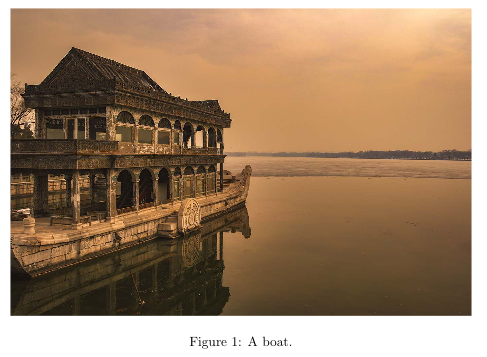
\includegraphics[width=0.5\linewidth]{_Graphics/boat1.png}
%  \caption{Example of a figure caption (the caption is placed below the figure).}
%  \label{fig:boat1}
%\end{figure}

%Figure \ref{fig:boat1} shows a boat.

%In the next page, I will create a table.
%\Begin{table}[h!]
%  \begin{center}
%    \caption{Table Caption.}
%    \label{tab:table1}
%    \begin{tabular}{l|l|r}
%      \textbf{Value 1} & \textbf{Value 2} & \textbf{Value 3}\\
%      $\alpha$ & $\beta$ & $\gamma$ \\
%      \hline
%      1 & 1110.1 & a\\
%      2 & 10.1 & b\\
%      3 & 23.113231 & c\\
%    \end{tabular}
%  \end{center}
%\end{table}

\nocite{*}
\bibliographystyle{IEEEtran} %the IEEtran file. You should not modify this file

\bibliography{IEEEabrv,references}

%references.bib is the name of the file where I wrote the references in .bib format


% that's all folks
\end{document}



%%% Local Variables:
%%% mode: latex
%%% TeX-master: t
%%% End:
